% 2008 年江西卷理科第 6 题：y=tan x+sin x-|tan x-sin x| 在 (π/2,3π/2) 内的四个候选图象。
% 来源 PDF：gaokaomath-src/普通高考/2008/2008江西文.pdf
% SHA-256：8d079d71fadf20911ed2fd71acfe9562b94eb962cfe5228fe7a376f3b599b239
% 原页：2008江西理.pdf 第 1 页（A3 三栏）第 1 栏，书页码 459。
% 绘制依据：由 |tan x - sin x| 分段，x∈(π/2,π) 时 y=2tan x（负值升到 0），
%   x∈(π,3π/2) 时 y=2sin x（由 0 降到 -2）。四个候选按原页 2×2 排布，
%   坐标刻度取 π/2→1、π→2、3π/2→3（单位长度相同），π/2 与 3π/2 的标号用白底压住虚线。
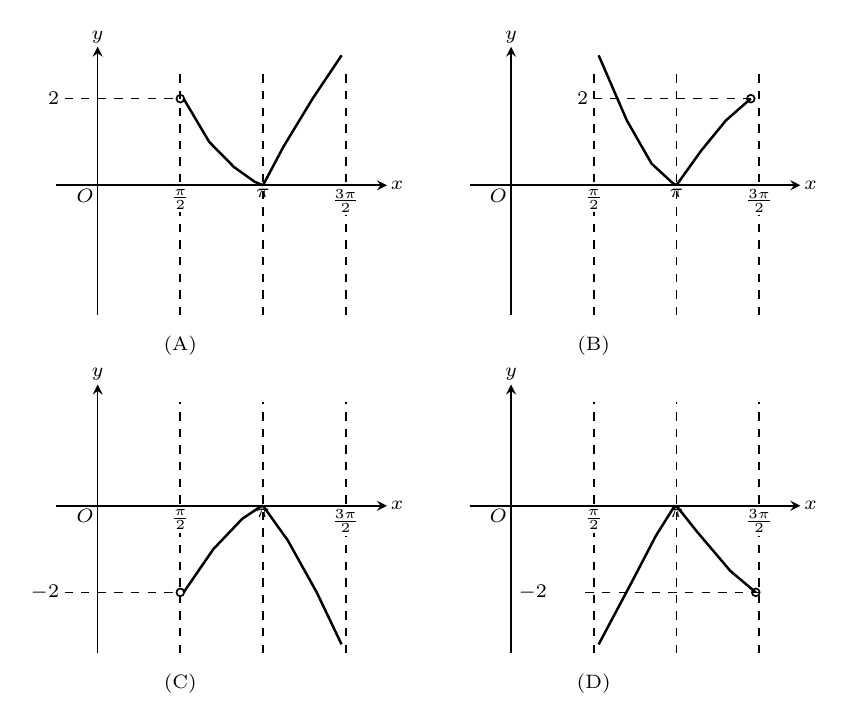
\begin{tikzpicture}[x=1.05cm, y=0.55cm, semithick, font=\scriptsize,
  every node/.style={inner sep=1.1pt}]

  % ---------- (A) ----------
  \begin{scope}[shift={(0,0)}]
    \draw[->,>=stealth] (-0.5,0) -- (3.5,0) node[right] {$x$};
    \draw[->,>=stealth] (0,-3.0) -- (0,3.2) node[above] {$y$};
    \node[below left] at (0,0) {$O$};
    \draw[dashed] (1.0,-3.0) -- (1.0,2.6);
    \draw[dashed] (2.0,-3.0) -- (2.0,2.6);
    \draw[dashed] (3.0,-3.0) -- (3.0,2.6);
    \node[below, fill=white] at (1.0,0) {$\frac{\pi}{2}$};
    \node[below] at (2.0,0) {$\pi$};
    \node[below, fill=white] at (3.0,0) {$\frac{3\pi}{2}$};
    \draw[dashed] (-0.4,2.0) -- (1.0,2.0);
    \node[left] at (-0.42,2.0) {$2$};
    \draw (1.0,2.0) circle (1.4pt);
    \draw[line width=0.9pt] plot coordinates {(1.04,2.0) (1.35,1.0) (1.65,0.42) (1.9,0.08) (2.0,0.0)};
    \draw[line width=0.9pt] plot coordinates {(2.0,0.0) (2.25,0.9) (2.6,2.0) (2.95,3.0)};
    \node at (1.0,-3.7) {(A)};
  \end{scope}

  % ---------- (B) ----------
  \begin{scope}[shift={(5.0,0)}]
    \draw[->,>=stealth] (-0.5,0) -- (3.5,0) node[right] {$x$};
    \draw[->,>=stealth] (0,-3.0) -- (0,3.2) node[above] {$y$};
    \node[below left] at (0,0) {$O$};
    \draw[dashed] (1.0,-3.0) -- (1.0,2.6);
    \draw[dashed] (2.0,-3.0) -- (2.0,2.6);
    \draw[dashed] (3.0,-3.0) -- (3.0,2.6);
    \node[below, fill=white] at (1.0,0) {$\frac{\pi}{2}$};
    \node[below] at (2.0,0) {$\pi$};
    \node[below, fill=white] at (3.0,0) {$\frac{3\pi}{2}$};
    \draw[dashed] (1.0,2.0) -- (2.9,2.0);
    \node[left] at (0.98,2.0) {$2$};
    \draw[line width=0.9pt] plot coordinates {(1.06,3.0) (1.4,1.5) (1.7,0.5) (1.95,0.06) (2.0,0.0)};
    \draw[line width=0.9pt] plot coordinates {(2.0,0.0) (2.3,0.8) (2.6,1.5) (2.9,2.0)};
    \draw (2.9,2.0) circle (1.4pt);
    \node at (1.0,-3.7) {(B)};
  \end{scope}

  % ---------- (C) ----------
  \begin{scope}[shift={(0,-7.4)}]
    \draw[->,>=stealth] (-0.5,0) -- (3.5,0) node[right] {$x$};
    \draw[->,>=stealth] (0,-3.4) -- (0,2.8) node[above] {$y$};
    \node[below left] at (0,0) {$O$};
    \draw[dashed] (1.0,-3.4) -- (1.0,2.4);
    \draw[dashed] (2.0,-3.4) -- (2.0,2.4);
    \draw[dashed] (3.0,-3.4) -- (3.0,2.4);
    \node[below, fill=white] at (1.0,0) {$\frac{\pi}{2}$};
    \node[below] at (2.0,0) {$\pi$};
    \node[below, fill=white] at (3.0,0) {$\frac{3\pi}{2}$};
    \draw[dashed] (-0.4,-2.0) -- (1.0,-2.0);
    \node[left] at (-0.42,-2.0) {$-2$};
    \draw (1.0,-2.0) circle (1.4pt);
    \draw[line width=0.9pt] plot coordinates {(1.04,-2.0) (1.4,-1.0) (1.75,-0.3) (1.97,-0.02) (2.0,0.0)};
    \draw[line width=0.9pt] plot coordinates {(2.0,0.0) (2.3,-0.8) (2.65,-2.0) (2.95,-3.2)};
    \node at (1.0,-4.1) {(C)};
  \end{scope}

  % ---------- (D) ----------
  \begin{scope}[shift={(5.0,-7.4)}]
    \draw[->,>=stealth] (-0.5,0) -- (3.5,0) node[right] {$x$};
    \draw[->,>=stealth] (0,-3.4) -- (0,2.8) node[above] {$y$};
    \node[below left] at (0,0) {$O$};
    \draw[dashed] (1.0,-3.4) -- (1.0,2.4);
    \draw[dashed] (2.0,-3.4) -- (2.0,2.4);
    \draw[dashed] (3.0,-3.4) -- (3.0,2.4);
    \node[below, fill=white] at (1.0,0) {$\frac{\pi}{2}$};
    \node[below] at (2.0,0) {$\pi$};
    \node[below, fill=white] at (3.0,0) {$\frac{3\pi}{2}$};
    \draw[dashed] (0.9,-2.0) -- (3.1,-2.0);
    \node[left] at (0.48,-2.0) {$-2$};
    \draw[line width=0.9pt] plot coordinates {(1.06,-3.2) (1.45,-1.8) (1.75,-0.7) (1.96,-0.06) (2.0,0.0)};
    \draw[line width=0.9pt] plot coordinates {(2.0,0.0) (2.25,-0.6) (2.65,-1.5) (2.96,-2.0)};
    \draw (2.96,-2.0) circle (1.4pt);
    \node at (1.0,-4.1) {(D)};
  \end{scope}
\end{tikzpicture}
